\documentclass[FIPLY_base.tex]{subfiles}

%\author{Daniel Bersenkowitsch}

\begin{document}
	\subsection{Begriffserklärung}
	Eine \grqq{}Wiederholung\grqq{} ist das 1-malige Ausüben einer Übung. 
	\newline
	Ein \grqq{}Satz\grqq{} umfasst alle Übungen und ausgeführten Wiederholungen.
	100\% RM =(Repetition Maximum = Maximalwiederholung) ist die Ausf"uhrung einer bestimmten "Uung zu einem bestimmten Gewicht, welches bei der "Ubung genau ein Mal bew"altigt werden kann:
	\[\%RM=\frac{100*Trainingsgewicht}{102.78-(2.78*Wiederholungen)}\]
	Wenn man sich also das Trainingsgewicht ausrechnen will, mit dem man eine "Ubung ausführen soll, geht man wie folgt vor (Vorgeschlagener \%RM-Wert und Wiederholungen sind angegeben):
	\[Trainingsgewicht=\frac{\%RM*(102.78-(2,78*Wiederholungen))}{100}\]
	Mit dem errechneten Gewicht führt man nun die jeweilige zugeordnete "Ubung aus. Da  bei konsequentem Training die Kraft steigt, sollte man auch immer das Trainingsgewicht erhöhen. Um maximalen Fortschritt zu erzielen, wird empfohlen, die Wiederholungen gleich bleiben zu lassen. Der Benutzer testet selbst wieviel Gewicht er mit den Wiederholungen schafft, die Änderung der Gewichts wird von ihm festgehalten, um positive Entwicklungen feststellen zu k"onnen. 
	\newline
	Das Gewicht kann auch selbst abgeschätzt werden. Das Gewicht ist dann optimal gewählt, wenn man damit zwischen 10 und 13 Wiederholungen schafft.
	Weiters wird immer auf eine Aufwärmphase hingewiesen, welche man vor jeder Trainingseinheit durchführen muss. Sie besteht aus 5-10 Minuten Laufen und Dehnen.
	
	\subsection{Einleitung}
	Ein Trainingsplan besteht aus unterschiedlichen Phasen - je nach Trainingsziel (Muskelaufbau, Maximalkraft, Kraftausdauer (=Gesundheit)) unterschiedlich. Jede Trainingsphase besitzt einen empfohlenenen RM-Wert (0\%-100\%), mit welchem der Benutzer "uben kann. Alle empfohlenen Werte (Satzpausen, RM-Wert, Anzahl der Trainingstage,...) sind jediglich eine Option für den Benutzer und können auch frei gewählt werden.
	Dabei zu bedenken ist, dass verschiedene Trainingsphasen bei verschiedenen Trainingsziele eine unterschiedliche Reihenfolge haben.
	Hier eine Visualisierung der Reihenfolge der Trainingsphasen:
	\begin{figure}[H]
		\centering
		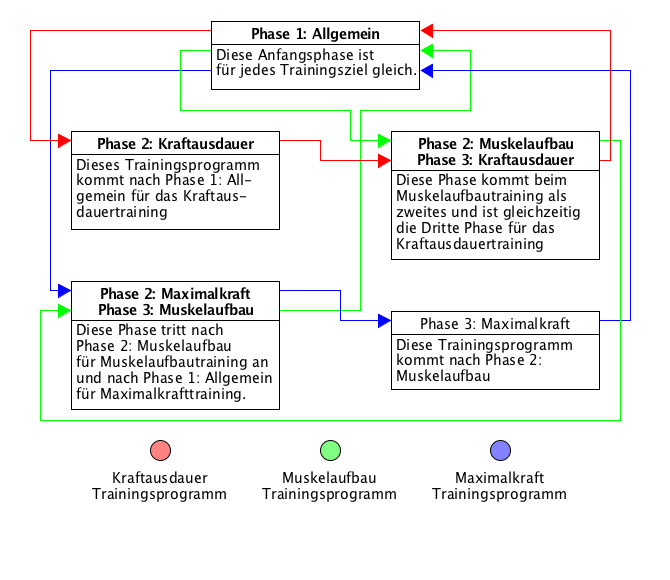
\includegraphics[scale=0.6]{img/VisualisierungTrainingsplan}
		\caption{Vorgangsvisualisierung der Trainingsplanphasen}
	\end{figure}
	
	\subsection{Phase 1: Allgemein}
	Phase 1 ist für jeden gleich, unabhängig vom Trainingsziel, und dient dem Eintrainieren. Am Anfang wird festgehalten, ob der Benutzer einen untrainierten oder bereits trainierten Körper besitzt. Anhand dessen und dem ausgewählten Schema (Bauch - Beine - Po, Oberkörper/Arme, Stabilisation (R"ucken \& Gesundheit)) werden in dieser Phase die "Ubungen ausgewählt und die Anzahl der S"atze/Wiederholungen bestimmt:
	\begin{center}
		\def\arraystretch{1.2}%
		\begin{tabular}{| l || l | l |}
			\hline
			 & \textbf{Anfänger} &\textbf{ Fortgeschrittener}\\
			\hline
			
			Baum - Beine - Po &  
				\begin{tabular}{ l  l }
					"Ubungen: & 9 \\
					S"atze: & 2 \\
					Wiederholungen: & 20 \\
				\end{tabular} & 
				\begin{tabular}{ l  l }
					"Ubungen: & 9 \\
					S"atze: & 3 \\
					Wiederholungen: & 25 \\
				\end{tabular} \\
			\hline
			Oberk"orper - Arme &
				\begin{tabular}{ l  l }
					"Ubungen: & 6 \\
					S"atze: & 2 \\
					Wiederholungen: & 20 \\
				\end{tabular} & 			
				\begin{tabular}{ l  l }
					"Ubungen: & 8 \\
					S"atze: & 3 \\
					Wiederholungen: & 25 \\
				\end{tabular} \\
			\hline
			Stabilisation & 
				\begin{tabular}{ l  l }
					"Ubungen: & 8 \\
					S"atze: & 2 \\
					Wiederholungen: & 20 \\
				\end{tabular} &
				\begin{tabular}{ l  l }
					"Ubungen: & 8 \\
					S"atze: & 3 \\
					Wiederholungen: & 25 \\
				\end{tabular} \\
				\hline
		\end{tabular}
	\end{center}
	In Phase 1 werden alle "Ubungen mit einem Gewicht 55\% RM ausgeführt. Es werden Anfangs 3 Trainingstage ausgewählt, an denen der Benutzer Zeit findet um zu trainieren. Dabei ist zu beachten, dass zwischen den Trainingstagen mind. 36 Stunden Pause eingelegt werden soll, um den Kreislauf zu schonen. Die empfohlene Satzpause liegt bei 30-60 Sekunden, kann aber auch frei bestimmt werden. \newline 
	Die Phase 1 dauert bei einem Anfänger 8 Wochen und bei einem Fortgeschrittenen nur die H"alfte.
	\newline
	Im "Uberblick:
		\begin{center}
			\def\arraystretch{1.3}%
			\begin{tabular}{| l | l |}
				\hline
				"Ubungen: & 6 bis 9 \\ \hline 
				Gewicht: & 55\% RM \\ \hline
				S"atze: & 2 oder 3 \\ \hline
				Wiederholungen: & 20 oder 25 \\ \hline
				Pausendauer: & 30-60 Sekunden \\ \hline
				Wochentage: & 3 \\ \hline
				Phasendauer: & 4 oder 8 Wochen \\ \hline
			\end{tabular} \\
		\end{center}
		
	\subsection{Phase 2: Kraftausdauer (Gesundheit)}
	Phase 2: Kraftausdauer (Gesundheit) besteht aus 2 "Phase 1: Allgemein Trainingstagen" in der Woche. Zusätzlich besteht das Training aus entweder ein Mal w"ochentlich Phase 2: Muskelaufbau -training oder ein Mal w"ochentlich Stabilit"ats"ubungen. Welche der Benutzer ausf"uhren will, kann er selbst am Anfang entscheiden, je nachdem ob er seinen K"orper formen will, oder ob er es als Gesundheits- oder Reha"ubung macht.
	\newline
	Also im "Uberblick:
	\newline
	\begin{center}
		\def\arraystretch{1.3}%
		\begin{tabular}{| l | l |}
			\hline
			1. Teil&Phase 1: Allgemein \\
			\hline
			"Ubungen: & 6 \\ \hline 
			Gewicht: & 55\% RM \\ \hline
			S"atze: & 2 \\ \hline
			Wiederholungen: & 25 \\ \hline
			Pausendauer: & 30-60 Sekunden \\ \hline
			Wochentage: & 2 \\ \hline
			Phasendauer: & 8 Wochen \\ \hline
		\end{tabular} 
	\end{center}
	\begin{center}
		\def\arraystretch{1.3}%
		\begin{tabular}{| l || l | l |}
			\hline
			 2. Teil & Phase 2: Muskelaufbau & Stabilit"ats"ubungen\\
			\hline
			"Ubungen: & 6  & 6\\ \hline 
			Gewicht: & 80\% RM & Keines \\ \hline
			S"atze: & 2 & 3 \\ \hline
			Wiederholungen: & 25 & 12-20 \\ \hline
			Pausendauer: & 30-60 Sekunden & 60-120 Sekunden \\ \hline
			Wochentage: & 1 & 1 \\ \hline
			Phasendauer: & 8 Wochen & 8 Wochen \\ \hline
		\end{tabular} 
	\end{center}
		
	\subsection{Phase 2: Muskelaufbau \newline Phase 3: Kraftausdauer}	
	Wenn man als Trainingsziel \grqq{}Muskelaufbau\grqq{} gewählt hat, kommt diese nach Phase 1, oder wenn man Phase 2: Kraftausdauer (Gesundheit) abgeschlossen hat. In dieser Phase kommt viel Hantel- und Seilzugtraining zum Einsatz. Dabei ist zu beachten, dass die Schwierigkeit der "Ubung egal ist. Es wird davon ausgegangen, dass ein Anf"anger nach der 8-w"ochigen Phase 1 bereits fit genug ist, um alle "Ubungen die sich im Trainingskatalog befinden zu meistern. 
	\newline
	Der User kann sich zu Beginn aussuchen, welche 2-3 Muskelgruppen er trainieren will. Am Phasenanfang wird zwischen Splittraining und Ganzkörpertraining unterschieden. Der Unterschied zwischen den Trainingsarten liegt bei der zeitlichen Ausführung der "Ubungen. Bei dem Splittraining werden "Ubungen zu einer bestimmten Muskelgruppe bei jeder Trainingseinheit durchgeführt. Umgekehrt wird bei dem Ganzk"orpertraining in jeder Trainingseinheit auf einen bestimmte Muskelgruppe geziehlt. 
	\newline
	Diese Phase besteht wieder aus 3 Trainingstagen pro Woche und das empfohlene Trainingsgewicht liegt bei 80\% RM. Die Satzpausendauer beträgt 90-120 Sekunden, bei 3 S"atzen und 12 Wiederholungen. Je nach Anzahl der fokusierten Muskelgruppen bestimmt sich die Zahl der "Ubungen, die man bekommt: Bei 2 Muskelbereiche sind es 6 "Ubungen, bei 3 sind es 9 "Ubungen. Nach dieser 8-wöchigen Phase kommt Phase 3: Muskelaufbau.
	\newline
	Im "Uberblick:
	\newline
	\begin{center}
		\def\arraystretch{1.3}%		
		\begin{tabular}{| l || l | l |}
			\hline
			& Muskelaufbau & Kraftausdauer \\ \hline
			"Ubungen: & 6 oder 9 & 6 oder 9 \\ \hline 
			Gewicht: & 80\% RM & 80\% RM \\ \hline
			S"atze: & 3 & 3\\ \hline
			Wiederholungen: & 12 & 12\\ \hline
			Pausendauer: & 90-120 Sekunden & 90-120 Sekunden \\ \hline
			Wochentage: & 3 & 3\\ \hline
			Phasendauer: & 8 Wochen & 4 Wochen \\ \hline
		\end{tabular} \\
	\end{center}
	Nach Phase 3: Kraftausdauer ist wieder von Anfang an (Phase 1: Allgemein) zu beginnen. Man kann aber auch aufh"oren oder sich einen neuen Trainingsplan generieren lassen.
	
	\subsection{Phase 2: Maximalkraft \newline Phase 3: Muskelaufbau}
	Diese Phase ist für das Maximalkrafttrainingsziel die Phase 2 und f"ur das Muskelaufbautrainingsziel die Phase 3. Nur Fortgeschrittene oder User die die Phase 2: Muskelaufbau durchgef"uhrt haben, k"onnen diese Phase beginnen.
	\newline
	Maximalkraft"ubungen sind immer Ganzk"orper"ubungen.
	Das empfohlene Trainingsgewicht liegt bei 95\% RM. Dabei kommen ausschließlich Seilzug- und Hantel"ubungen vor (6). Satzdauer beträgt 90-120 Sekunden, bei 3 S"atzen und 5 Wiederholungen. Diese Phase besteht wieder aus 3 Trainingstagen pro Woche und einer Mindesterholungszeit von 48h!
	\newline
	Das Maximalkrafttraining besteht aus einem zusätzlichen Schritt, der Mobilisation, die nach dem Aufwärmen beginnt. Danach kann mit dem Training begonnen werden.
	\newline
	Im "Uberblick:
		\begin{center}
			\def\arraystretch{1.3}%
			\begin{tabular}{| l | l |}
				\hline
				"Ubungen: & 6 \\ \hline 
				Gewicht: & 95\% RM \\ \hline
				S"atze: & 3 \\ \hline
				Wiederholungen: & 5 \\ \hline
				Pausendauer: & 90-120 Sekunden \\ \hline
				Wochentage: & 3 \\ \hline
				Phasendauer: & 
				\begin{tabular}{l l}
					Muskelaufbau: & 4 Wochen \\ 
					Maximalkraft: & 6 Wochen \\
				\end{tabular} \\ \hline
			\end{tabular} \\ 
		\end{center}
	Nach Phase 3: Muskelaufbau ist der Trainingsplan zu ende. Nun kann man ihn erneut starten (vom Anfang an), h"ort auf, oder l"asst sich erneut einen generieren.
	
	\subsection{Phase 3: Maximalkraft}
	Phase 3: Maximalkraft kommt nach Phase 2: Maximalkraft. Hierbei wird jediglich 2 Mal w"ochentlich trainiert. Die Tage kann sich der Benutzer wieder aussuchen, einzige Bedingung sind 48 Stunden Erholungszeit. 
	Die Phase besteht wieder aus Seilzug- und Hantel"ubungen, insgesamt 6 mit jeweils 2 Wiederholungen zu 5 Sätzen. Hierbei wird das Trainingsgewicht erneut f"ur ca. 95\%RM gew"ahlt.
	\newline
	Im "Uberblick: 
		\begin{center}
			\def\arraystretch{1.3}%
			\begin{tabular}{| l | l |}
				\hline
				"Ubungen: & 6 \\ \hline 
				Gewicht: & 95\% RM \\ \hline
				S"atze: & 5 \\ \hline
				Wiederholungen: & 2 \\ \hline
				Pausendauer: & 120-180 Sekunden \\ \hline
				Wochentage: & 2 \\ \hline
				Phasendauer: & 8 Wochen \\ \hline
			\end{tabular} 
		\end{center}
	Nach Phase 3: Maximalkraft ist der Trainingsplan zu Ende. Nun kann man ihn erneut starten (vom Anfang an), h"ort auf, oder l"asst sich erneut einen generieren.
	
	\subsection{Mobilisation}
	Die Mobilisation beim Maximalkrafttraining dient dazu, den K"orper auf das kommende schwere Training vorzubereiten. 
	Sie besteht aus:
			\begin{center}
				\begin{tabular}{ p{5cm} | p{8cm} }
					\hline
					\ \\
					\textbf{Mobilisation} & \textbf{Beschreibung}     
					\\ \hline \hline
					\ \\ 
					Becken-Mob & \pbox{10cm}{Die Arme über den Köpf führen, Handflächen \newline nach oben schieben, Schultern bleiben tief, \newline das Becken im Uhrzeigersinn, den ganzen \newline Bewegungsumfang ausnutzen, Richtung \newline ändern, die Kreise aus der Hüfte führen, die \newline Beine sind stabil.}
					\ \\ 
					\\ \hline
					\ \\
					Wirbelsäule – Seitneigung & \pbox{10cm}{Linken Arm seitwärts hoch heben über den \newline Kopf und Wirbelsäule seitwärts beugen, \newline gegengleich, Handflächen nach oben.}
					\ \\ 
					\ \\
					\hline
					\ \\
					Wirbelsäule – Rotation & \pbox{10cm}{Bauchnabel nach innen ziehen, die Arme in \newline U-Form anheben, Daumen zeigen nach hinten \newline und sind leicht nach außen gedreht, den \newline Oberkörper vorbeugen, Gesäß nach hinten \newline und zur Seite drehen, zur Mitte kommen, zur \newline anderen Seite drehen, zur Mitte, immer im \newline Wechsel, der Rücken bleibt gestreckt, die \newline Schulterblätter sind zusammengezogen, \newline das Becken bleibt stabil.}
					\ \\ 
					\\ \hline
					\ \\
					Wirbelsäule – Rolldown & \pbox{10cm}{Aufrechter Stand, den Kopf Richtung \newline Brustbein senken, Bauchnabel nach innen \newline ziehen, einatmen und beim Ausatmen die \newline Wirbelsäule Wirbel für Wirbel in Richtung \newline Boden abrollen, einatmen und wieder Wirbel \newline für Wirbel aufrollen, der Rücken ist locker, \newline der Nacken ist entspannt.}
					\ \\
					\\ \hline
				\end{tabular} 
			\end{center}
			\begin{center}
				\begin{tabular}{ p{5cm} | p{8cm} }
					\hline
					\ \\
					\textbf{Mobilisation} & \textbf{Beschreibung}     
					\\ \hline \hline
					\ \\
					Hals & \pbox{10cm}
					{Den Kopf im Wechsel nach rechts und links \newline drehen.}
					\ \\ 
					\\ \hline
					\ \\ 					
					Schulter & \pbox{10cm}{Die Arme neben dem Körper hängen lassen \newline und mit den Schultern nach rückwärts kreisen.}
					\ \\ 
					\\ \hline
					\ \\
					Ellbogen & \pbox{10cm}{Die Hände auf die Schulter legen, mit den\newline Ellbogen vorwärts und rückwärts kreisen, \newline die Schultern dabei nach hinten und unten \newline bewegen.}
					\ \\ 
					\\ \hline
					\ \\ 
					Handgelenk & \pbox{10cm}{Hände kreisen, beide Hände gleichzeitig mit \newline größtmöglichem Bewegungsumfang \newline fortlaufend um die eigene Achse drehen.}
					\ \\ 
					\\ \hline
					\ \\ 
				\end{tabular} 
			\end{center}

[\citetitle{tplantheorie} \cite{tplantheorie}]
\end{document}